\section{Andmejälgija} \label{Andmejälgija}

\subsection{The protocol} \label{protocol_desc}

Andmejälgija is a protocol that state databases are responsible for implementing themselves. In order for the database to offer an \textit{Andmejälgija} service, they have to create an X-Road interface according to RIA specification\cite{aj-github-spec}. 

X-Road is a REST-based protocol which is used for secure data exchange between Estonian information systems over the Internet.

The \textit{Andmejälgija} X-Road interface is expected to have the following endpoints:

\textbf{\texttt{findUsage}}

A query searches the data recorder database for usage records that match the constraints given in the input. The output of the query returns all records found\cite{aj-github-spec}.

\textbf{\texttt{usagePeriod}}

The time period for which usage information can be requested\cite{aj-github-spec}.

\textbf{\texttt{heartbeat}}

Requesting the availability status of the tracker's usage information\cite{aj-github-spec}.

The overall architecture of the \textit{Andmejälgija} system is illustrated in Figure~\ref{fig:aj-model}, which shows how state databases interact with the \textit{eesti.ee} portal through X-Road to provide data access logs to end users.

\begin{figure}[H]
\centering
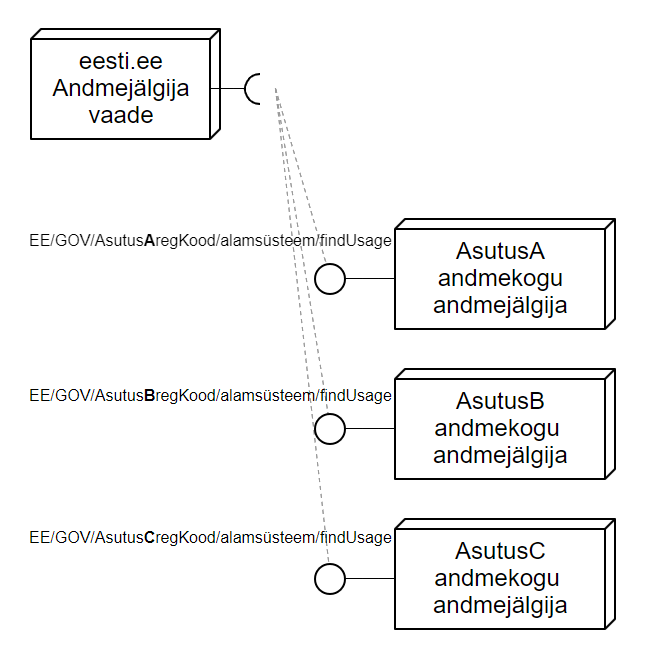
\includegraphics[width=450px]{english/figures/aj_model.PNG}
\caption{\textit{Andmejälgija} (Data Tracker) system architecture showing the interaction between entities implementing data tracking and \textit{eesti.ee} Data Tracker view. The data exchange happens via X-Road\cite{aj-github}.}
\label{fig:aj-model}
\end{figure}

\subsection{Usage}
There are several ways for end-users to access their Data Tracker data. State portal \textit{eesti.ee} provides a web-view for \textit{Andmejälgija} where end users can access their data access logs. Recently, RIA have also published a mobile application for \textit{eesti.ee}, that also features a view of data access logs. 

Another way to access Data tracker data is through Estonian Population Registry, although, is seems to be Population Registry specific as it doesn't provide access logs from other databases



\subsection{Adoption}
The current adoption of \textit{Andmejälgija} has some noticeable issues. Very often it is not at all clear why your data have been accessed, at least from the first glance. Explanation messages are vague and confusing, often being similar to ``data access by personal code'', making it difficult to understand the reason behind the data access, even if it was you who accessed it.

There is even an information sheet with recommendations for services implementing the \textit{Andmejälgija} protocol, and it states that providing poor quality explanations for data access is a bad practice\cite{ria-andmejalgija-recommendations}. The good and poor examples of data access descriptions are shown in Table~\ref{tab:example-good} and Table~\ref{tab:example-bad}.

\textbf{Good practice example:}

\begin{table}[H]
\centering
\begin{tabular}{|p{3cm}|p{6cm}|p{4cm}|}
\hline
\textbf{Data Processing Time} & \textbf{Activity} & \textbf{Party Receiving Personal Data} \\
\hline
13.01.2015 10:20:27 & Prescription viewed by doctor; prescription number 1018472350 & Doctor Viktor Pihlakas \\
\hline
19.01.2018 10:58:23 & Individual query for valid driver's licenses through state portal \textit{eesti.ee} & Jaan Kask 32405023456 \\
\hline
\end{tabular}
\caption{Example of good data access descriptions\cite{ria-andmejalgija-recommendations}}
\label{tab:example-good}
\end{table}

\textbf{Bad practice example:}

\begin{table}[H]
\centering
\begin{tabular}{|p{3cm}|p{6cm}|p{4cm}|}
\hline
\textbf{Data Processing Time} & \textbf{Activity} & \textbf{Party Receiving Personal Data} \\
\hline
13.01.2015 10:20:27 & PERSONAL DATA BY PERSONAL CODE & INSTITUTION X \\
\hline
19.01.2018 10:58:23 & INDIVIDUAL EXTENDED INFO QUERY BY PERSONAL CODE & FOUNDATION Y \\
\hline
\end{tabular}
\caption{Example of poor data access descriptions\cite{ria-andmejalgija-recommendations}}
\label{tab:example-bad}
\end{table}

Apparently, the advice is often ignored, as many institutions tend to follow the bad example in practice. The thesis author's Data Tracker view is flooded with entries containing poor quality descriptions like those shown in Table~\ref{tab:author-data-tracker}.

\begin{table}[H]
\centering
\begin{tabular}{|p{2.5cm}|p{5cm}|p{3cm}|p{3.5cm}|}
\hline
\textbf{Date \& Time} & \textbf{Institution} & \textbf{Database} & \textbf{Activity} \\
\hline
02.08.2025 11:15 & Health and Welfare Information Systems Centre & Population Registry & INDIVIDUAL EXTENDED INFO QUERY BY PERSONAL CODE \\
\hline
01.08.2025 22:37 & Health and Welfare Information Systems Centre & Population Registry & INDIVIDUAL NAME RETRIEVAL BASED ON PERSONAL CODE \\
\hline
01.08.2025 20:23 & Education and Youth Board & Population Registry & PERSONAL DATA BY PERSONAL CODE \\
\hline
\end{tabular}
\caption{Extract from author's Data Tracker view demonstrating poor quality descriptions}
\label{tab:author-data-tracker}
\end{table}

Furthermore, currently there is no law requiring institutions to implement the \textit{Andmejälgija} protocol, meaning that its use is essentially voluntary. This may change in the future, however, as the current coalition government formed by the Estonian Reform Party and Eesti 200 has promised to make the use of \textit{Andmejälgija} compulsory according to their coalition agreement\cite{coalition-agreement-2025-2027}.

In the following chapters I will cover different state databases and their implementations of \textit{Andmejälgija}, and whether they implement the protocol at all.